\section{Application dédié}
\paragraph{}
Nous avons opté à exploiter ce réseau de neurones avec une application mobile qui traduit le langage des signes en mots. L’application se connecte avec un gant qui contient des marqueurs. Ce dernier envoi à l’application les positions des marqueurs en utilisant des accéléromètres pour qu’elle puisse reconnaitre le geste effectué afin de le traduire.

Pour simuler une telle application, nous avons codé les lettres latins avec des combinaisons des cinq gestes reconnus par le réseau de neurones.\\
\begin{center}
	\begin{figure}[H]
		\centering
		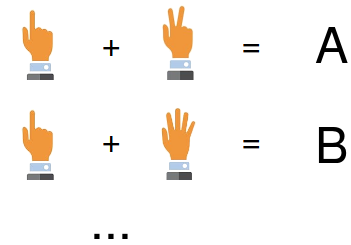
\includegraphics[scale=0.4]{images/coding.png}
		\caption{\small Codage des lettres latins en utilisant les gestes}
	\end{figure}
\end{center}
\subsection{Schéma de l’application}
\paragraph{}
L’application se devise en deux parties:
\begin{itemize}[label=\textbullet]
	\item Une pour simuler localement la traduction, c’est à dire elle utilise des données de testes déjà prêtes.
	\item L’autre recherche un gant sur le réseau, et récupère les données de ce dernier.
	Pour réaliser cette partie nous utilisons une application desktop pour simuler le gant afin d’envoyer les données à l’application. 
\end{itemize}
\begin{center}
	\begin{figure}[H]
		\centering
		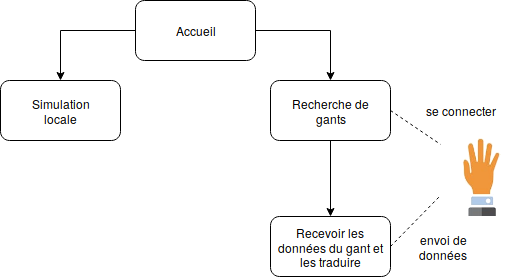
\includegraphics[scale=0.67]{images/Schema.png}
		\caption{\small Schéma générale de l’application}
	\end{figure}
\end{center}


